\documentclass[12pt]{article}
\usepackage{url, graphicx, epstopdf}

% page layout
\setlength{\topmargin}{-0.25in}
\setlength{\textheight}{9.5in}
\setlength{\headheight}{0in}
\setlength{\headsep}{0in}
\setlength{\parindent}{1.1\baselineskip}

% problem formatting
\newcommand{\problemname}{Problem}
\newcounter{problem}

% words
\newcommand{\foreign}[1]{\textsl{#1}}
\newcommand{\vs}{\foreign{vs}}

% math
\newcommand{\dd}{\mathrm{d}}
\newcommand{\e}{\mathrm{e}}

% primary units
\newcommand{\rad}{\mathrm{rad}}
\newcommand{\kg}{\mathrm{kg}}
\newcommand{\m}{\mathrm{m}}
\newcommand{\s}{\mathrm{s}}

% secondary units
\renewcommand{\deg}{\mathrm{deg}}
\newcommand{\km}{\mathrm{km}}
\newcommand{\cm}{\mathrm{cm}}
\newcommand{\mm}{\mathrm{mm}}
\newcommand{\ft}{\mathrm{ft}}
\newcommand{\mi}{\mathrm{mi}}
\newcommand{\AU}{\mathrm{AU}}
\newcommand{\ns}{\mathrm{ns}}
\newcommand{\h}{\mathrm{h}}
\newcommand{\yr}{\mathrm{yr}}
\newcommand{\N}{\mathrm{N}}
\newcommand{\J}{\mathrm{J}}
\newcommand{\eV}{\mathrm{eV}}
\newcommand{\W}{\mathrm{W}}
\newcommand{\Pa}{\mathrm{Pa}}

% derived units
\newcommand{\mps}{\m\,\s^{-1}}
\newcommand{\mph}{\mi\,\h^{-1}}
\newcommand{\mpss}{\m\,\s^{-2}}

% random stuff
\sloppy\sloppypar\raggedbottom\frenchspacing\thispagestyle{empty}

\begin{document}

\section*{NYU Physics I---rolling}

A heavy round pipe of mass $m$, radius $R$, and moment of inertia $I$
sits at rest on the horizontal bed of a parked truck, a distance $L$
from the end of the truck bed.  It isn't properly secured!

At time $t=0$, the truck starts to
accelerate forwards with acceleration $a$, at which point the pipe
begins to roll without slipping on the truck bed.  Give all your
answers with respect to the stationary ground, {\em not} the moving
truck. \\ \rule{0.3\textwidth}{0pt}
\resizebox{0.4\textwidth}{!}{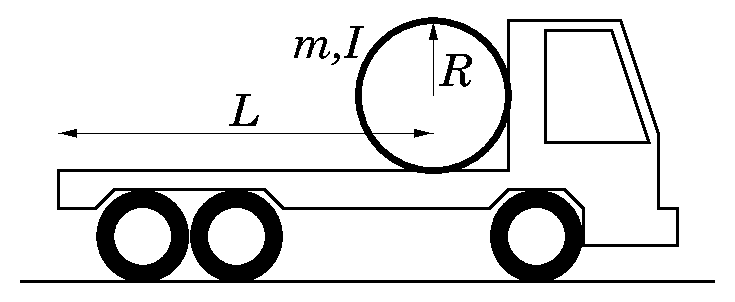
\includegraphics{truckpipe.eps}}

\textsl{(a)} Forget the truck for a moment. Imagine you have a pipe
of radius $R$ rolling (without slipping) on the ground at (center-of-mass) speed $v$ with
respect to the ground. What is the relationship between the speed $v$ of the pipe
and the angular speed $\omega$ of the pipe and why?

\textsl{(b)} Now, back to the truck:
During the acceleration, when the truck is moving at
speed $v_t$ and the pipe is moving at speed $v_p$ (with respect to the
ground) and the pipe is spinning at angular speed $\omega_p$, what is
the condition (that is, the equation relating $v_t$, $v_p$, $\omega_p$
and $R$) for rolling without slipping on the truck bed?  \emph{Think
about the movement of the pipe relative to the truck bed.}

\textsl{(c)} Draw a free body diagram for the pipe, showing all
forces, for $t>0$.

\textsl{(d)} Which way does the pipe accelerate (relative to the
ground)?  Will its acceleration be greater or less than $a$?  Which
way does it start to spin?  That is, anticipate the dynamics.

\textsl{(e)} What is the acceleration of the pipe?  That is, solve the
equations you have.

\textsl{(f)} (Optional!) When (at what time) does the pipe fall off the truck?

\end{document}
